\section{Technische Realisierung}
In diesem Kapitel gehen wir auf die technische Realisierung des Projektes ein. Im Abschnitt Domänenmodell werden zunächst die verwendeten Begriffe definiert. Anschließend wird auf die Architektur, das Datenmodell und die Authentifizierung der Benutzerrollen eingegangen. Abschließend beschreiben wir exemplarisch einen Methodenaufruf, mit dem die wichtigsten Komponenten des Systems vorgestellt werden.

\subsection{Domänenmodell}



Roles:
Admin: 
Verwaltet die Songs auf dem Server
Party People:
Voten die Songs
Ist nach dem ersten Kontakt eindeutig identifizierbar (Party People ID)
Jukebox: datenbankgestützte Wildfly-Anwendung
Verwaltung der Songs und Song-Informationen
Songs hinzufügen
Songs löschen 
Song-Informationen bearbeiten
Generierung und Verwaltung der Playlist
Song
Hat Song-Information
Muss abspielbar sein
Pfad in Dateisystem
Internetstream
YouTube-Link
Song-Information:
Titel, Interpret, Genre, Album, Länge
Current Song:
Song der gerade gespielt wird.
Wenn Current Song abgespielt ist, wird der erste Song aus der Playlist entfernt und zum Current Song.
Playlist:
Absteigend sortierte Song Liste auf Basis des Votings
Playlist wird durch Playlist-Füll-Prozess generiert:
Solange Größe Playlist nicht erreicht, wähle nächsten Song via Song-Selection
Song-Selection
Nächste Song wird auf Basis von DI, Party Time usw. ausgewählt
Aus globaler Song Liste der Jukebox
Voting
Basiert auf Playlist
Erlaubt Party People Songs innerhalb der Playlist zu bewerten:
Up-Vote
Down-Vote
Vote v = Anzahl Up-Votes - Anzahl Down-Votes
Party People darf pro Song max. einmal voten
DI:
Beschreibt den Betrunkenheitsgrad der Party People
ganzzahliger Wert zw. 0 - 100


\subsection{Architektur}
- Systemübersicht / Komponentendiagramm
- Beans und deren Aufgaben


\subsection{Datenmodell}

- Kasten stellen Entity-Beans dar
- Pfeile stellen die Beziehungen (Unidirektional, bidirektional) dar
- Zwischen den Pfeilen stehen die Cascading Types

\begin{figure}[H]
\centering
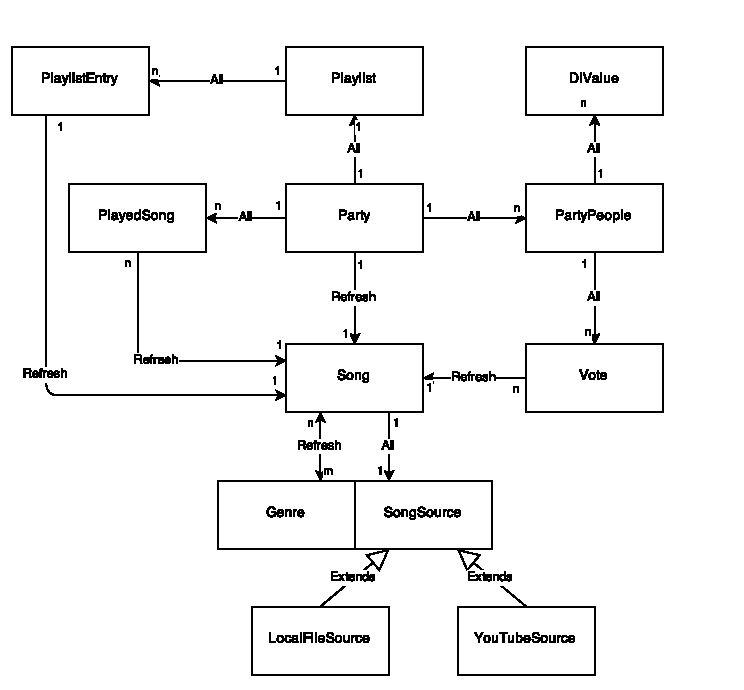
\includegraphics[width=1\linewidth]{Bilder/EntityBeansModelMitCascading}
\caption{}
\label{fig:EntityBeansModelMitCascading}
\end{figure}


\subsection{Benutzerrollen}
ggf. umbenennen in Authentifizierung oder Authentifizierung der Benutzerrollen
- Authentifizierung via Datenbank im Wildfly
- Schritte zur Realisierung
- Aufführung der Probleme


\subsection{Exemplarische Darstellung}

- Beschreibung eines Funktionsaufrufes z.B. start Party durch alle "`Schichten"' des Systems



